%%! TEX program = xelatex
\documentclass[varwidth=20.5cm,border=4]{standalone}
\usepackage{fontspec}
\usepackage{grffile}
\usepackage{graphicx}
\usepackage{caption}
\usepackage[labelformat=empty,position=top]{subcaption}
\usepackage[export]{adjustbox}
\setmainfont{Arial}

\captionsetup{labelformat=empty}

\begin{document}

\begin{figure}[tb]
    \large
    %\centering
    \begin{subfigure}[t]{0.3\linewidth}
        \textbf{A}
        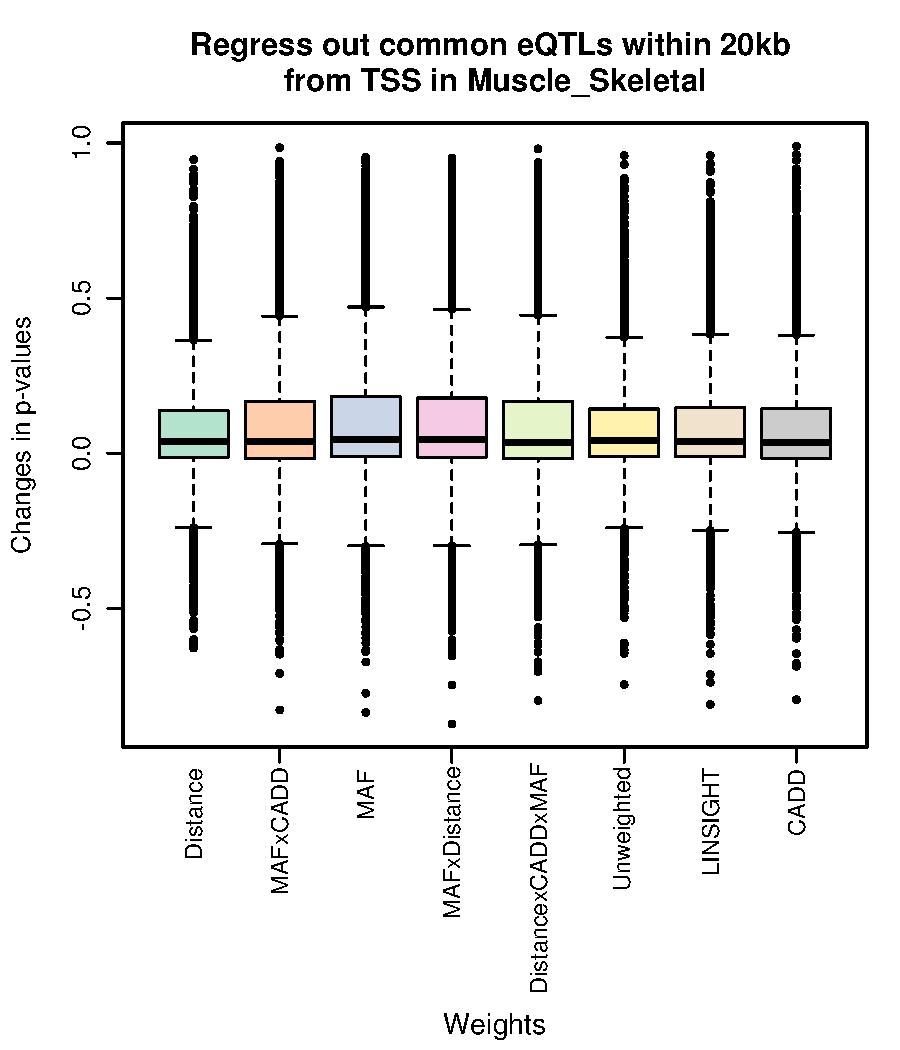
\includegraphics[width=0.9\linewidth,valign=t]{./changes.p.values.Muscle_Skeletal.20kb.pdf}
    \end{subfigure}
	\hspace{0.1cm}

    \begin{subfigure}[t]{0.3\linewidth}
        \textbf{B}
        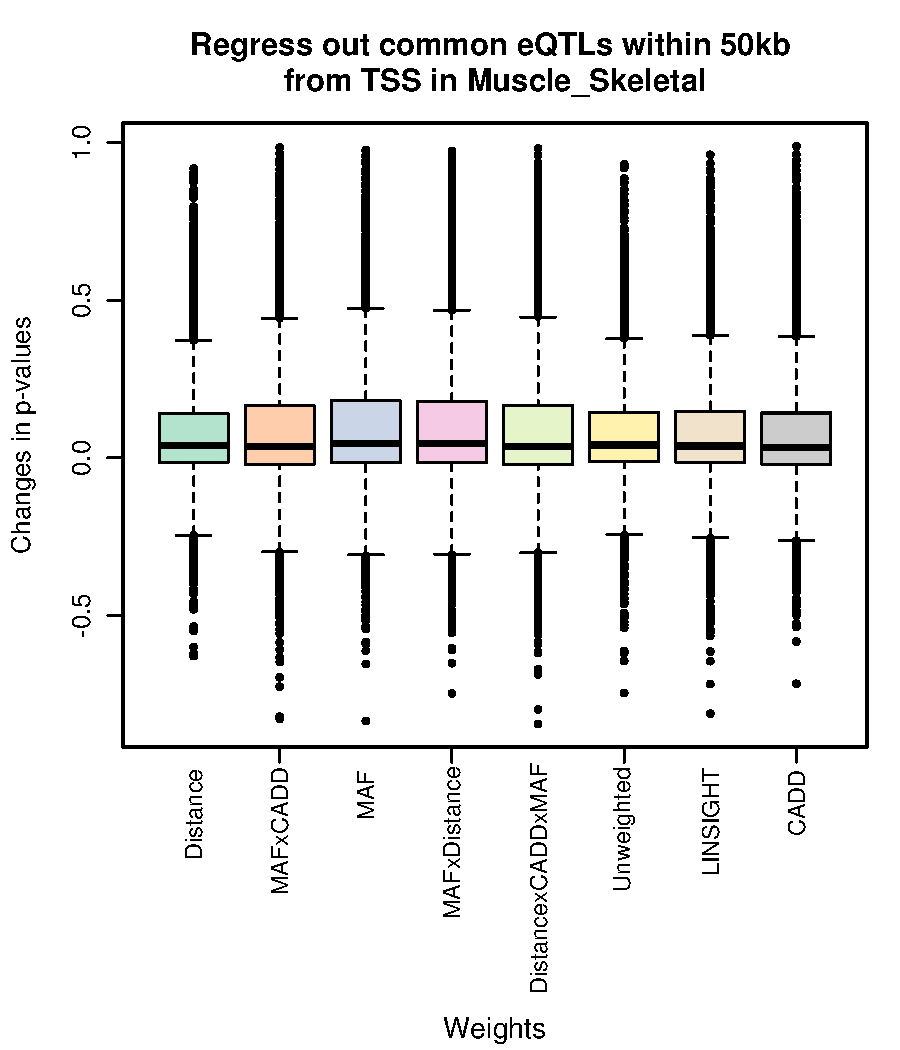
\includegraphics[width=0.9\linewidth,valign=t]{./changes.p.values.Muscle_Skeletal.50kb.pdf}
    \end{subfigure}
	\hspace{0.1cm}

    \begin{subfigure}[t]{0.3\linewidth}
        \textbf{C}
        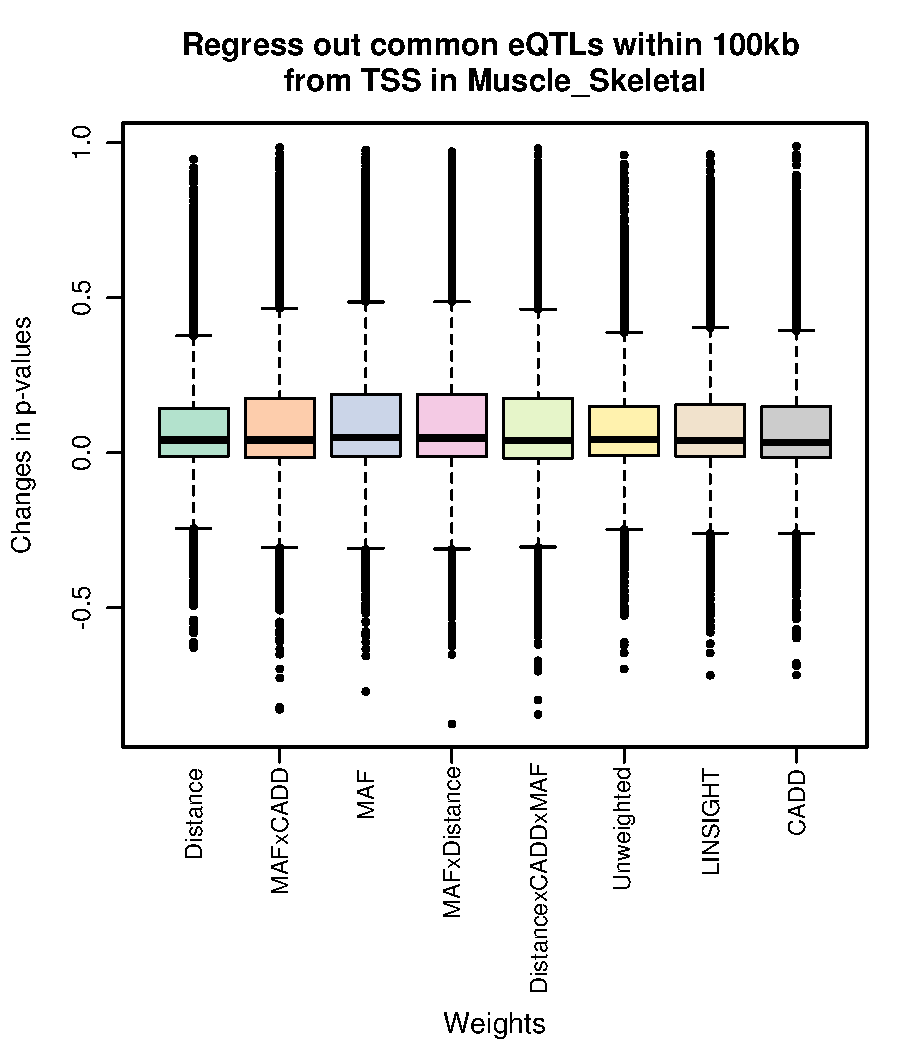
\includegraphics[width=0.9\linewidth,valign=t]{./changes.p.values.Muscle_Skeletal.100kb.pdf}
    \end{subfigure}
%	\hspace{0.1cm}

    \begin{subfigure}[t]{0.3\linewidth}
        \textbf{A}
        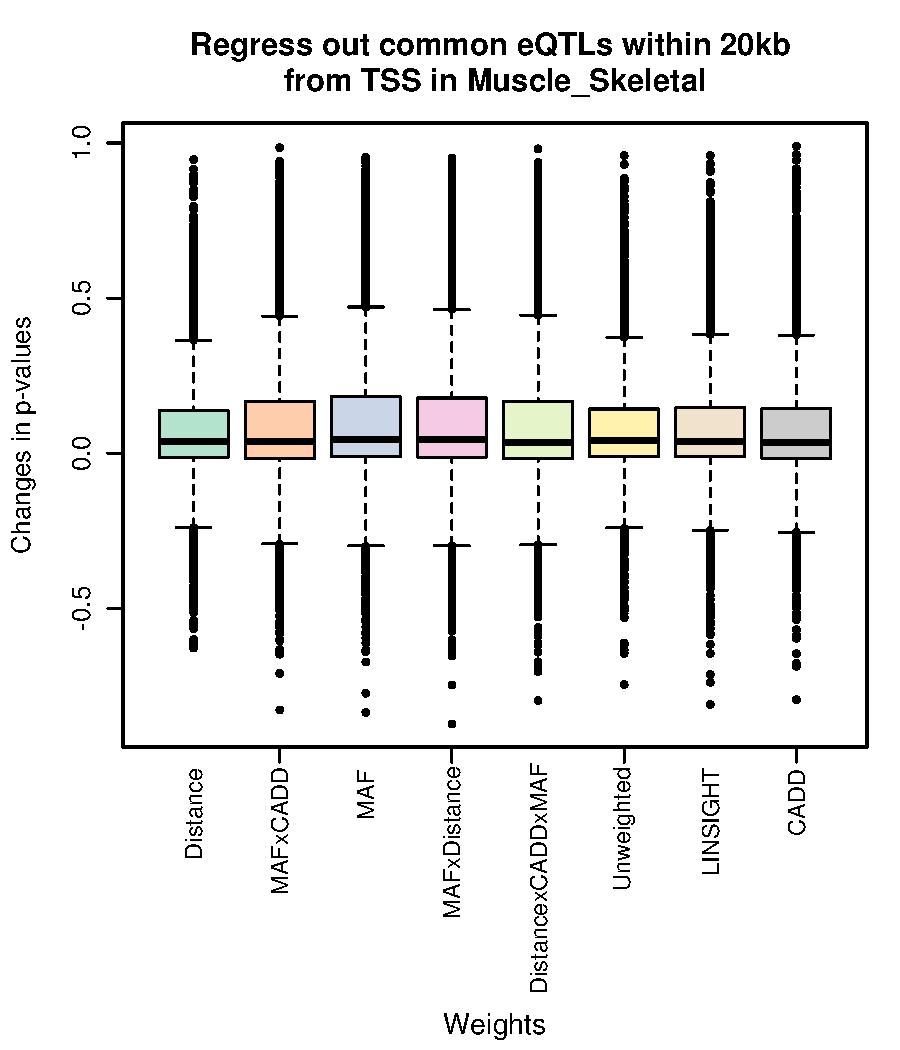
\includegraphics[width=0.9\linewidth,valign=t]{./changes.p.values.Muscle_Skeletal.20kb.pdf}
    \end{subfigure}

    \begin{subfigure}[t]{0.3\linewidth}
        \textbf{A}
        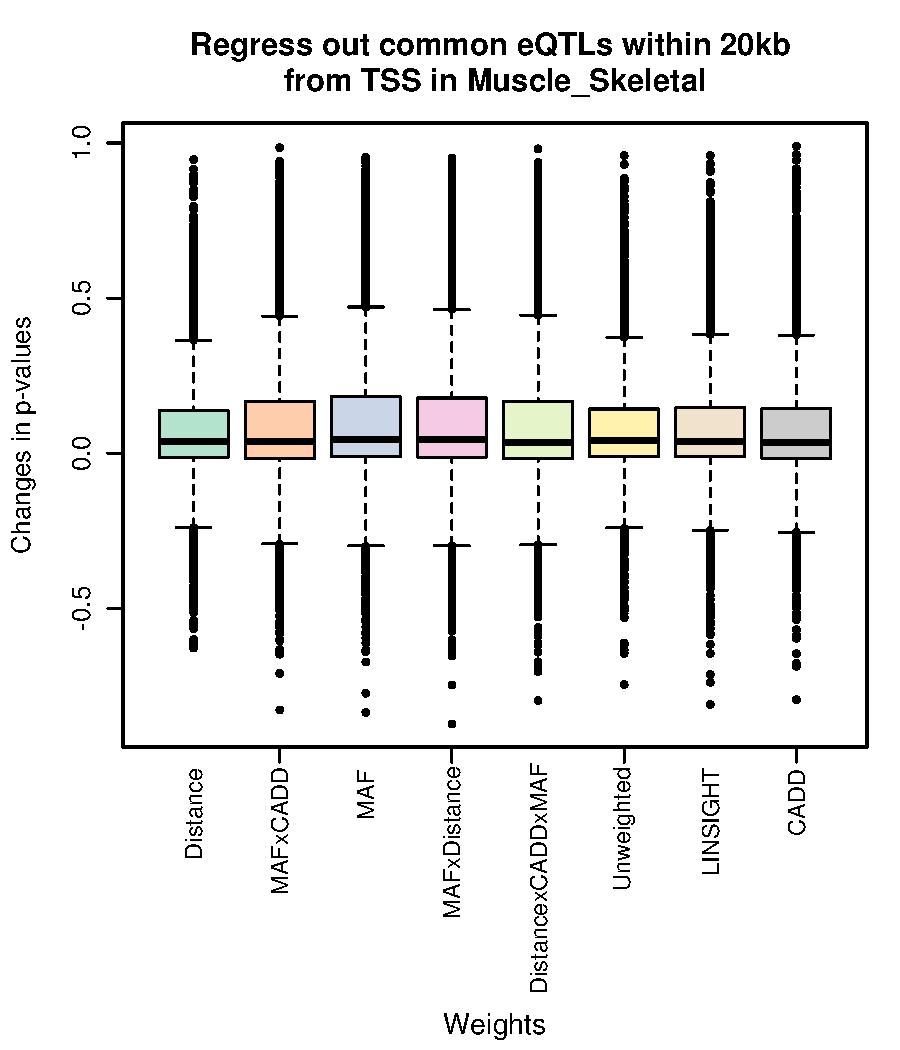
\includegraphics[width=0.9\linewidth,valign=t]{./changes.p.values.Muscle_Skeletal.20kb.pdf}
    \end{subfigure}


\end{figure}
\end{document}
